\documentclass[twoside]{book}

% Packages required by doxygen
\usepackage{fixltx2e}
\usepackage{calc}
\usepackage{doxygen}
\usepackage[export]{adjustbox} % also loads graphicx
\usepackage{graphicx}
\usepackage[utf8]{inputenc}
\usepackage{makeidx}
\usepackage{multicol}
\usepackage{multirow}
\PassOptionsToPackage{warn}{textcomp}
\usepackage{textcomp}
\usepackage[nointegrals]{wasysym}
\usepackage[table]{xcolor}

% Font selection
\usepackage[T1]{fontenc}
\usepackage[scaled=.90]{helvet}
\usepackage{courier}
\usepackage{amssymb}
\usepackage{sectsty}
\renewcommand{\familydefault}{\sfdefault}
\allsectionsfont{%
  \fontseries{bc}\selectfont%
  \color{darkgray}%
}
\renewcommand{\DoxyLabelFont}{%
  \fontseries{bc}\selectfont%
  \color{darkgray}%
}
\newcommand{\+}{\discretionary{\mbox{\scriptsize$\hookleftarrow$}}{}{}}

% Page & text layout
\usepackage{geometry}
\geometry{%
  a4paper,%
  top=2.5cm,%
  bottom=2.5cm,%
  left=2.5cm,%
  right=2.5cm%
}
\tolerance=750
\hfuzz=15pt
\hbadness=750
\setlength{\emergencystretch}{15pt}
\setlength{\parindent}{0cm}
\setlength{\parskip}{3ex plus 2ex minus 2ex}
\makeatletter
\renewcommand{\paragraph}{%
  \@startsection{paragraph}{4}{0ex}{-1.0ex}{1.0ex}{%
    \normalfont\normalsize\bfseries\SS@parafont%
  }%
}
\renewcommand{\subparagraph}{%
  \@startsection{subparagraph}{5}{0ex}{-1.0ex}{1.0ex}{%
    \normalfont\normalsize\bfseries\SS@subparafont%
  }%
}
\makeatother

% Headers & footers
\usepackage{fancyhdr}
\pagestyle{fancyplain}
\fancyhead[LE]{\fancyplain{}{\bfseries\thepage}}
\fancyhead[CE]{\fancyplain{}{}}
\fancyhead[RE]{\fancyplain{}{\bfseries\leftmark}}
\fancyhead[LO]{\fancyplain{}{\bfseries\rightmark}}
\fancyhead[CO]{\fancyplain{}{}}
\fancyhead[RO]{\fancyplain{}{\bfseries\thepage}}
\fancyfoot[LE]{\fancyplain{}{}}
\fancyfoot[CE]{\fancyplain{}{}}
\fancyfoot[RE]{\fancyplain{}{\bfseries\scriptsize Generated by Doxygen }}
\fancyfoot[LO]{\fancyplain{}{\bfseries\scriptsize Generated by Doxygen }}
\fancyfoot[CO]{\fancyplain{}{}}
\fancyfoot[RO]{\fancyplain{}{}}
\renewcommand{\footrulewidth}{0.4pt}
\renewcommand{\chaptermark}[1]{%
  \markboth{#1}{}%
}
\renewcommand{\sectionmark}[1]{%
  \markright{\thesection\ #1}%
}

% Indices & bibliography
\usepackage{natbib}
\usepackage[titles]{tocloft}
\setcounter{tocdepth}{3}
\setcounter{secnumdepth}{5}
\makeindex

% Hyperlinks (required, but should be loaded last)
\usepackage{ifpdf}
\ifpdf
  \usepackage[pdftex,pagebackref=true]{hyperref}
\else
  \usepackage[ps2pdf,pagebackref=true]{hyperref}
\fi
\hypersetup{%
  colorlinks=true,%
  linkcolor=blue,%
  citecolor=blue,%
  unicode%
}

% Custom commands
\newcommand{\clearemptydoublepage}{%
  \newpage{\pagestyle{empty}\cleardoublepage}%
}

\usepackage{caption}
\captionsetup{labelsep=space,justification=centering,font={bf},singlelinecheck=off,skip=4pt,position=top}

%===== C O N T E N T S =====

\begin{document}

% Titlepage & ToC
\hypersetup{pageanchor=false,
             bookmarksnumbered=true,
             pdfencoding=unicode
            }
\pagenumbering{alph}
\begin{titlepage}
\vspace*{7cm}
\begin{center}%
{\Large Secure Text Editor \\[1ex]\large 2.\+0.\+0 }\\
\vspace*{1cm}
{\large Generated by Doxygen 1.8.14}\\
\end{center}
\end{titlepage}
\clearemptydoublepage
\pagenumbering{roman}
\tableofcontents
\clearemptydoublepage
\pagenumbering{arabic}
\hypersetup{pageanchor=true}

%--- Begin generated contents ---
\chapter{Hierarchical Index}
\section{Class Hierarchy}
This inheritance list is sorted roughly, but not completely, alphabetically\+:\begin{DoxyCompactList}
\item \contentsline{section}{Crypto\+Manager}{\pageref{class_crypto_manager}}{}
\item \contentsline{section}{File\+Manager}{\pageref{class_file_manager}}{}
\item \contentsline{section}{Model}{\pageref{class_model}}{}
\item Application\begin{DoxyCompactList}
\item \contentsline{section}{App}{\pageref{class_app}}{}
\end{DoxyCompactList}
\end{DoxyCompactList}

\chapter{Class Index}
\section{Class List}
Here are the classes, structs, unions and interfaces with brief descriptions\+:\begin{DoxyCompactList}
\item\contentsline{section}{\mbox{\hyperlink{class_app}{App}} }{\pageref{class_app}}{}
\item\contentsline{section}{\mbox{\hyperlink{class_crypto_manager}{Crypto\+Manager}} }{\pageref{class_crypto_manager}}{}
\item\contentsline{section}{\mbox{\hyperlink{class_file_manager}{File\+Manager}} }{\pageref{class_file_manager}}{}
\item\contentsline{section}{\mbox{\hyperlink{class_model}{Model}} }{\pageref{class_model}}{}
\end{DoxyCompactList}

\chapter{File Index}
\section{File List}
Here is a list of all files with brief descriptions\+:\begin{DoxyCompactList}
\item\contentsline{section}{Secure Text Editor v2/src/\mbox{\hyperlink{_app_8java}{App.\+java}} }{\pageref{_app_8java}}{}
\item\contentsline{section}{Secure Text Editor v2/src/\mbox{\hyperlink{_crypto_manager_8java}{Crypto\+Manager.\+java}} }{\pageref{_crypto_manager_8java}}{}
\item\contentsline{section}{Secure Text Editor v2/src/\mbox{\hyperlink{_file_manager_8java}{File\+Manager.\+java}} }{\pageref{_file_manager_8java}}{}
\item\contentsline{section}{Secure Text Editor v2/src/\mbox{\hyperlink{_model_8java}{Model.\+java}} }{\pageref{_model_8java}}{}
\end{DoxyCompactList}

\chapter{Class Documentation}
\hypertarget{class_app}{}\section{App Class Reference}
\label{class_app}\index{App@{App}}
Inheritance diagram for App\+:\begin{figure}[H]
\begin{center}
\leavevmode
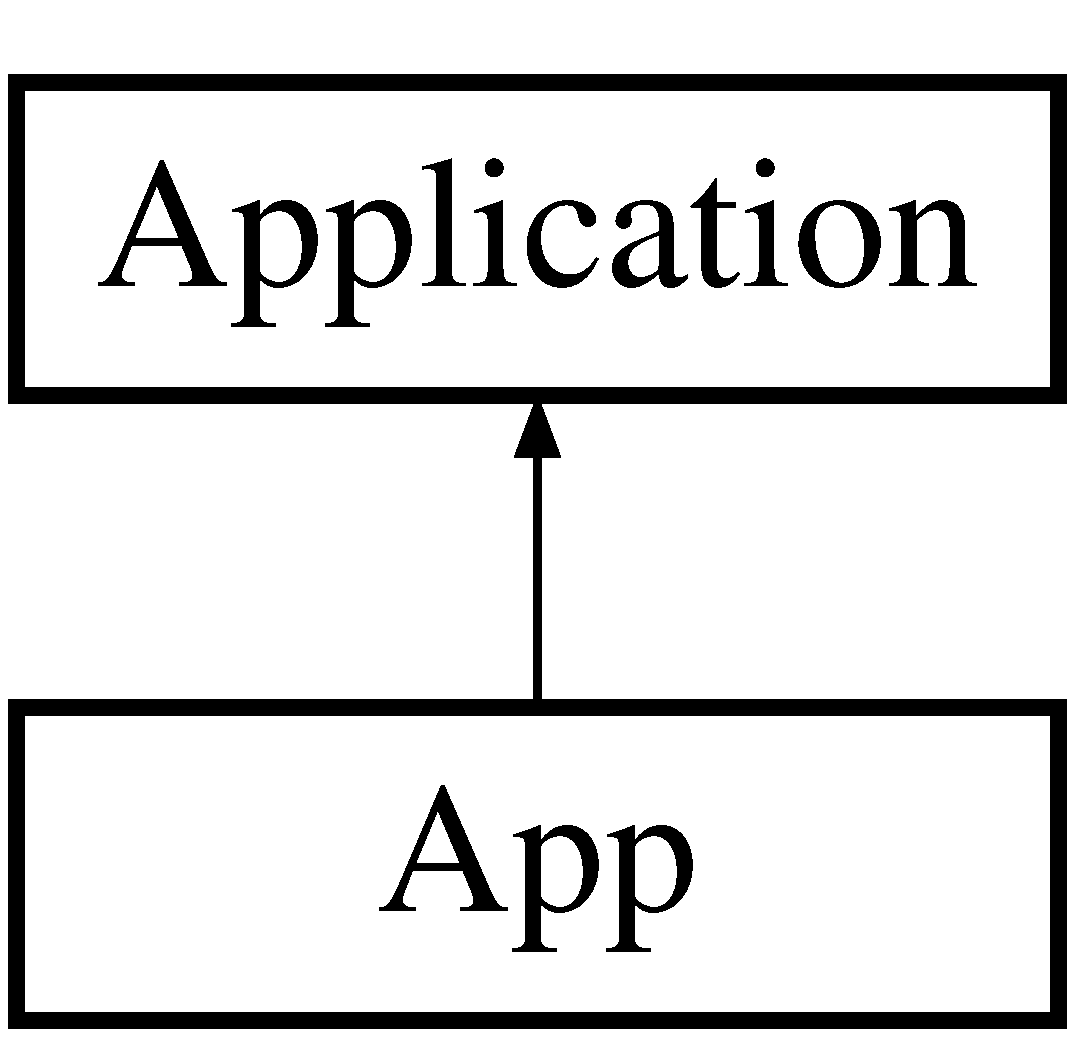
\includegraphics[height=2.000000cm]{class_app}
\end{center}
\end{figure}
\subsection*{Public Member Functions}
\begin{DoxyCompactItemize}
\item 
void \mbox{\hyperlink{class_app_a1e9bed8a34c642bf9796dc6ba51ad2b6}{start}} (Stage stage)  throws Exception 
\item 
void \mbox{\hyperlink{class_app_ac05e2e5c6881f45164dba0662e9741ee}{open\+Encryption\+Window}} ()
\end{DoxyCompactItemize}
\subsection*{Static Public Member Functions}
\begin{DoxyCompactItemize}
\item 
static void \mbox{\hyperlink{class_app_a941972c4be68395f473d23f1cbf101a7}{main}} (String\mbox{[}$\,$\mbox{]} args)
\end{DoxyCompactItemize}


\subsection{Member Function Documentation}
\mbox{\Hypertarget{class_app_a941972c4be68395f473d23f1cbf101a7}\label{class_app_a941972c4be68395f473d23f1cbf101a7}} 
\index{App@{App}!main@{main}}
\index{main@{main}!App@{App}}
\subsubsection{\texorpdfstring{main()}{main()}}
{\footnotesize\ttfamily static void App.\+main (\begin{DoxyParamCaption}\item[{String \mbox{[}$\,$\mbox{]}}]{args }\end{DoxyParamCaption})\hspace{0.3cm}{\ttfamily [static]}}

\mbox{\Hypertarget{class_app_ac05e2e5c6881f45164dba0662e9741ee}\label{class_app_ac05e2e5c6881f45164dba0662e9741ee}} 
\index{App@{App}!open\+Encryption\+Window@{open\+Encryption\+Window}}
\index{open\+Encryption\+Window@{open\+Encryption\+Window}!App@{App}}
\subsubsection{\texorpdfstring{open\+Encryption\+Window()}{openEncryptionWindow()}}
{\footnotesize\ttfamily void App.\+open\+Encryption\+Window (\begin{DoxyParamCaption}{ }\end{DoxyParamCaption})}

Manages encryption window G\+UI.

On first call it creates the stage, any calls later simply display the scene. \mbox{\Hypertarget{class_app_a1e9bed8a34c642bf9796dc6ba51ad2b6}\label{class_app_a1e9bed8a34c642bf9796dc6ba51ad2b6}} 
\index{App@{App}!start@{start}}
\index{start@{start}!App@{App}}
\subsubsection{\texorpdfstring{start()}{start()}}
{\footnotesize\ttfamily void App.\+start (\begin{DoxyParamCaption}\item[{Stage}]{stage }\end{DoxyParamCaption}) throws Exception}

Create G\+UI and start it 

The documentation for this class was generated from the following file\+:\begin{DoxyCompactItemize}
\item 
Secure Text Editor v2/src/\mbox{\hyperlink{_app_8java}{App.\+java}}\end{DoxyCompactItemize}

\hypertarget{class_crypto_manager}{}\section{Crypto\+Manager Class Reference}
\label{class_crypto_manager}\index{Crypto\+Manager@{Crypto\+Manager}}
\subsection*{Static Public Member Functions}
\begin{DoxyCompactItemize}
\item 
static byte \mbox{[}$\,$\mbox{]} \mbox{\hyperlink{class_crypto_manager_a16c99441e20ceb5e1e6bb20abdc33f24}{encrypt}} (String input, Encryption\+Type encryption, Mode\+Type mode, Padding\+Type padding)  throws Exception 
\item 
static String \mbox{\hyperlink{class_crypto_manager_a63fce196907289e0568b8d0bde582be0}{decrypt}} (byte\mbox{[}$\,$\mbox{]} input, Encryption\+Type encryption, Mode\+Type mode, Padding\+Type padding)  throws Exception 
\end{DoxyCompactItemize}


\subsection{Member Function Documentation}
\mbox{\Hypertarget{class_crypto_manager_a63fce196907289e0568b8d0bde582be0}\label{class_crypto_manager_a63fce196907289e0568b8d0bde582be0}} 
\index{Crypto\+Manager@{Crypto\+Manager}!decrypt@{decrypt}}
\index{decrypt@{decrypt}!Crypto\+Manager@{Crypto\+Manager}}
\subsubsection{\texorpdfstring{decrypt()}{decrypt()}}
{\footnotesize\ttfamily static String Crypto\+Manager.\+decrypt (\begin{DoxyParamCaption}\item[{byte \mbox{[}$\,$\mbox{]}}]{input,  }\item[{Encryption\+Type}]{encryption,  }\item[{Mode\+Type}]{mode,  }\item[{Padding\+Type}]{padding }\end{DoxyParamCaption}) throws Exception\hspace{0.3cm}{\ttfamily [static]}}

Decrypts a byte array to a String using various encryption methods, modes and padding types by making use of the Bouncy\+Castle -\/ provider. 
\begin{DoxyParams}{Parameters}
{\em input} & to decryptable byte array \\
\hline
{\em encryption} & Encryption Method \\
\hline
{\em mode} & Mode \\
\hline
{\em padding} & Padding \\
\hline
\end{DoxyParams}
\begin{DoxyReturn}{Returns}
Encrypted String. 
\end{DoxyReturn}

\begin{DoxyExceptions}{Exceptions}
{\em Exception} & \\
\hline
\end{DoxyExceptions}
\mbox{\Hypertarget{class_crypto_manager_a16c99441e20ceb5e1e6bb20abdc33f24}\label{class_crypto_manager_a16c99441e20ceb5e1e6bb20abdc33f24}} 
\index{Crypto\+Manager@{Crypto\+Manager}!encrypt@{encrypt}}
\index{encrypt@{encrypt}!Crypto\+Manager@{Crypto\+Manager}}
\subsubsection{\texorpdfstring{encrypt()}{encrypt()}}
{\footnotesize\ttfamily static byte \mbox{[}$\,$\mbox{]} Crypto\+Manager.\+encrypt (\begin{DoxyParamCaption}\item[{String}]{input,  }\item[{Encryption\+Type}]{encryption,  }\item[{Mode\+Type}]{mode,  }\item[{Padding\+Type}]{padding }\end{DoxyParamCaption}) throws Exception\hspace{0.3cm}{\ttfamily [static]}}

Encrypts a String to a byte array using various encryption methods, modes and padding types by making use of the Bouncy\+Castle -\/ provider.


\begin{DoxyParams}{Parameters}
{\em input} & To encryptable string. \\
\hline
{\em encryption} & Encryption Method \\
\hline
{\em mode} & Encryption Mode \\
\hline
{\em padding} & Padding \\
\hline
\end{DoxyParams}
\begin{DoxyReturn}{Returns}
encrypted byte array 
\end{DoxyReturn}


The documentation for this class was generated from the following file\+:\begin{DoxyCompactItemize}
\item 
Secure Text Editor v2/src/\mbox{\hyperlink{_crypto_manager_8java}{Crypto\+Manager.\+java}}\end{DoxyCompactItemize}

\hypertarget{class_file_manager}{}\section{File\+Manager Class Reference}
\label{class_file_manager}\index{File\+Manager@{File\+Manager}}
\subsection*{Static Public Member Functions}
\begin{DoxyCompactItemize}
\item 
static String \mbox{\hyperlink{class_file_manager_a52f2989a90be68d1632274d84a165030}{open\+From\+Path}} (String path, Encryption\+Type encryption, Mode\+Type mode, Padding\+Type padding)
\item 
static void \mbox{\hyperlink{class_file_manager_a44f1be89277979c7e729562bbedd3145}{save\+To\+Path}} (File file, String input, Encryption\+Type encryption, Mode\+Type mode, Padding\+Type padding)
\end{DoxyCompactItemize}


\subsection{Member Function Documentation}
\mbox{\Hypertarget{class_file_manager_a52f2989a90be68d1632274d84a165030}\label{class_file_manager_a52f2989a90be68d1632274d84a165030}} 
\index{File\+Manager@{File\+Manager}!open\+From\+Path@{open\+From\+Path}}
\index{open\+From\+Path@{open\+From\+Path}!File\+Manager@{File\+Manager}}
\subsubsection{\texorpdfstring{open\+From\+Path()}{openFromPath()}}
{\footnotesize\ttfamily static String File\+Manager.\+open\+From\+Path (\begin{DoxyParamCaption}\item[{String}]{path,  }\item[{Encryption\+Type}]{encryption,  }\item[{Mode\+Type}]{mode,  }\item[{Padding\+Type}]{padding }\end{DoxyParamCaption})\hspace{0.3cm}{\ttfamily [static]}}

Reads a byte array from a given path to then decrypt it using the \mbox{\hyperlink{class_crypto_manager}{Crypto\+Manager}} class.


\begin{DoxyParams}{Parameters}
{\em path} & Path to read the file from. \\
\hline
{\em encryption} & Encryption Method \\
\hline
{\em mode} & Mode \\
\hline
{\em padding} & Padding type \\
\hline
\end{DoxyParams}
\begin{DoxyReturn}{Returns}
Encrypted content from file as String 
\end{DoxyReturn}
\mbox{\Hypertarget{class_file_manager_a44f1be89277979c7e729562bbedd3145}\label{class_file_manager_a44f1be89277979c7e729562bbedd3145}} 
\index{File\+Manager@{File\+Manager}!save\+To\+Path@{save\+To\+Path}}
\index{save\+To\+Path@{save\+To\+Path}!File\+Manager@{File\+Manager}}
\subsubsection{\texorpdfstring{save\+To\+Path()}{saveToPath()}}
{\footnotesize\ttfamily static void File\+Manager.\+save\+To\+Path (\begin{DoxyParamCaption}\item[{File}]{file,  }\item[{String}]{input,  }\item[{Encryption\+Type}]{encryption,  }\item[{Mode\+Type}]{mode,  }\item[{Padding\+Type}]{padding }\end{DoxyParamCaption})\hspace{0.3cm}{\ttfamily [static]}}

Encrypts an input String using the \mbox{\hyperlink{class_crypto_manager}{Crypto\+Manager}} class to then write it to a file.


\begin{DoxyParams}{Parameters}
{\em file} & The output file \\
\hline
{\em input} & The input String \\
\hline
{\em encryption} & Encryption Method \\
\hline
{\em mode} & Mode \\
\hline
{\em padding} & Padding type \\
\hline
\end{DoxyParams}


The documentation for this class was generated from the following file\+:\begin{DoxyCompactItemize}
\item 
Secure Text Editor v2/src/\mbox{\hyperlink{_file_manager_8java}{File\+Manager.\+java}}\end{DoxyCompactItemize}

\hypertarget{class_model}{}\section{Model Class Reference}
\label{class_model}\index{Model@{Model}}
\subsection*{Public Member Functions}
\begin{DoxyCompactItemize}
\item 
\mbox{\hyperlink{class_model_adc740be264b0c173c4574f42361f1e3a}{Model}} (Text\+Area text\+Area)
\item 
void \mbox{\hyperlink{class_model_a7e8201067bda1c35b779490c46b9590c}{set\+Encryption\+Type}} (Encryption\+Type encryption)
\item 
void \mbox{\hyperlink{class_model_a7b6d65f0bdf44c6d91267b917662fa0c}{set\+Mode\+Type}} (Mode\+Type mode)
\item 
void \mbox{\hyperlink{class_model_ad173621b4a9b3242952a63379062818a}{set\+Padding\+Type}} (Padding\+Type padding)
\end{DoxyCompactItemize}


\subsection{Constructor \& Destructor Documentation}
\mbox{\Hypertarget{class_model_adc740be264b0c173c4574f42361f1e3a}\label{class_model_adc740be264b0c173c4574f42361f1e3a}} 
\index{Model@{Model}!Model@{Model}}
\index{Model@{Model}!Model@{Model}}
\subsubsection{\texorpdfstring{Model()}{Model()}}
{\footnotesize\ttfamily Model.\+Model (\begin{DoxyParamCaption}\item[{Text\+Area}]{text\+Area }\end{DoxyParamCaption})}

Constructor 

\subsection{Member Function Documentation}
\mbox{\Hypertarget{class_model_a7e8201067bda1c35b779490c46b9590c}\label{class_model_a7e8201067bda1c35b779490c46b9590c}} 
\index{Model@{Model}!set\+Encryption\+Type@{set\+Encryption\+Type}}
\index{set\+Encryption\+Type@{set\+Encryption\+Type}!Model@{Model}}
\subsubsection{\texorpdfstring{set\+Encryption\+Type()}{setEncryptionType()}}
{\footnotesize\ttfamily void Model.\+set\+Encryption\+Type (\begin{DoxyParamCaption}\item[{Encryption\+Type}]{encryption }\end{DoxyParamCaption})}

Setter Method for Encryption\+Type \mbox{\Hypertarget{class_model_a7b6d65f0bdf44c6d91267b917662fa0c}\label{class_model_a7b6d65f0bdf44c6d91267b917662fa0c}} 
\index{Model@{Model}!set\+Mode\+Type@{set\+Mode\+Type}}
\index{set\+Mode\+Type@{set\+Mode\+Type}!Model@{Model}}
\subsubsection{\texorpdfstring{set\+Mode\+Type()}{setModeType()}}
{\footnotesize\ttfamily void Model.\+set\+Mode\+Type (\begin{DoxyParamCaption}\item[{Mode\+Type}]{mode }\end{DoxyParamCaption})}

Setter Method for Mode\+Type \mbox{\Hypertarget{class_model_ad173621b4a9b3242952a63379062818a}\label{class_model_ad173621b4a9b3242952a63379062818a}} 
\index{Model@{Model}!set\+Padding\+Type@{set\+Padding\+Type}}
\index{set\+Padding\+Type@{set\+Padding\+Type}!Model@{Model}}
\subsubsection{\texorpdfstring{set\+Padding\+Type()}{setPaddingType()}}
{\footnotesize\ttfamily void Model.\+set\+Padding\+Type (\begin{DoxyParamCaption}\item[{Padding\+Type}]{padding }\end{DoxyParamCaption})}

Setter Method for Padding\+Type 

The documentation for this class was generated from the following file\+:\begin{DoxyCompactItemize}
\item 
Secure Text Editor v2/src/\mbox{\hyperlink{_model_8java}{Model.\+java}}\end{DoxyCompactItemize}

\chapter{File Documentation}
\hypertarget{_app_8java}{}\section{Secure Text Editor v2/src/\+App.java File Reference}
\label{_app_8java}\index{Secure Text Editor v2/src/\+App.\+java@{Secure Text Editor v2/src/\+App.\+java}}
\subsection*{Classes}
\begin{DoxyCompactItemize}
\item 
class \mbox{\hyperlink{class_app}{App}}
\end{DoxyCompactItemize}

\hypertarget{_crypto_manager_8java}{}\section{Secure Text Editor v2/src/\+Crypto\+Manager.java File Reference}
\label{_crypto_manager_8java}\index{Secure Text Editor v2/src/\+Crypto\+Manager.\+java@{Secure Text Editor v2/src/\+Crypto\+Manager.\+java}}
\subsection*{Classes}
\begin{DoxyCompactItemize}
\item 
class \mbox{\hyperlink{class_crypto_manager}{Crypto\+Manager}}
\end{DoxyCompactItemize}

\hypertarget{_file_manager_8java}{}\section{Secure Text Editor v2/src/\+File\+Manager.java File Reference}
\label{_file_manager_8java}\index{Secure Text Editor v2/src/\+File\+Manager.\+java@{Secure Text Editor v2/src/\+File\+Manager.\+java}}
\subsection*{Classes}
\begin{DoxyCompactItemize}
\item 
class \mbox{\hyperlink{class_file_manager}{File\+Manager}}
\end{DoxyCompactItemize}

\hypertarget{_model_8java}{}\section{Secure Text Editor v2/src/\+Model.java File Reference}
\label{_model_8java}\index{Secure Text Editor v2/src/\+Model.\+java@{Secure Text Editor v2/src/\+Model.\+java}}
\subsection*{Classes}
\begin{DoxyCompactItemize}
\item 
class \mbox{\hyperlink{class_model}{Model}}
\end{DoxyCompactItemize}

%--- End generated contents ---

% Index
\backmatter
\newpage
\phantomsection
\clearemptydoublepage
\addcontentsline{toc}{chapter}{Index}
\printindex

\end{document}
